\documentclass[10pt,aspectratio=43]{beamer}
	\usetheme[sectionpages]{UniNA}

	\usepackage[utf8]{inputenc}
	\usepackage[english]{babel}
	\usepackage[T1]{fontenc}
	\usepackage{csquotes}

	\usepackage[scaled]{beramono}
	\usepackage[scale=1.05]{AlegreyaSans}
	\usepackage{beamer_shortcuts}
	\usetikzlibrary{spy}
	\usepackage[backend=biber, citetracker=true, style=numeric]{biblatex}
	\addbibresource{../report/bibliography.bib}

	\title[Regularization via Bidualization] %shown at the top of frames
	{Sparse Regularization via Bidualization} %shown in title frame
	\subtitle{Based on the article of Amir Beck and Yehonathan Refael}

	\date{October, 2020} %explicitly set date instead of \today

	\author[]%shown at the top of frames
	{%shown in title frame
		{Lefort Tanguy}%
	}

	\institute[
	]
	{% is placed on the bottom of the title page
	    University of Montpellier
	}

\begin{document}
	\maketitle

%%%%%%%%%%%%%%%%%%%%%%%%%%%
% Table of contents
%%%%%%%%%%%%%%%%%%%%%%%%%%%
	\begin{frame}{Content}{}
		\tableofcontents
	\end{frame}

%%%%%%%%%%%%%%%%%%%%%%%%%%%%%%%%%%%%%%%%%%%
%%%%%%%%%%%%%% Introduction %%%%%%%%%%%%%%%
%%%%%%%%%%%%%%%%%%%%%%%%%%%%%%%%%%%%%%%%%%%

\section{Introduction}
\begin{frame}{Introduction}{Solve problems with regularizations}
We want to solve:
\begin{onlyenv}<1>
\[\arg\min_{x\in\RR^n} \|Ax-b\|^2  \]
\end{onlyenv}

\begin{onlyenv}<2->
\[\arg\min_{x\in\RR^n} \|Ax-b\|^2 \color{red}+ \mathrm{pen}(x)\]

What we wish for a penalty:
\begin{itemize}
    \item convexity (a unique solution, use the inequality, \dots),
    \item continuity,
    \item differentiability.
\end{itemize}
\end{onlyenv}
\end{frame}

% Different types of regularizations

\begin{frame}{Introduction}{With a sparse setting...}

    \begin{itemize}
        \item<1-> Tikhonov-Ridge regularization:    $\quad\|Ax-b\|^2 + \frac{\lambda}{2}\|x\|_2^2\enspace,$
        \item<2-> LASSO:
        $\quad\frac{1}{2}\|Ax-b\|^2_2 + \lambda \|x\|_1\enspace,$
        \item<3-> Elastic-net:
        $\quad\frac{1}{2}\|Ax-b\|^2_2 + \lambda_1 \|x\|_1 +  \frac{\lambda_2}{2}\|x\|^2_2\enspace.$
        \end{itemize}
        \begin{onlyenv}<4->
\begin{figure}[ht]\centering
\caption{Comparison of the \lasso and \enet estimation of the sparse signal with highly correlated groups of variables.}
\vspace{-.1cm}

\begin{tikzpicture}[
    zoomboxarray,
    zoomboxarray columns=1,
    zoomboxarray rows=2,
    connect zoomboxes,
    zoombox paths/.append style={line width=1pt}
]
    \node [image node] { 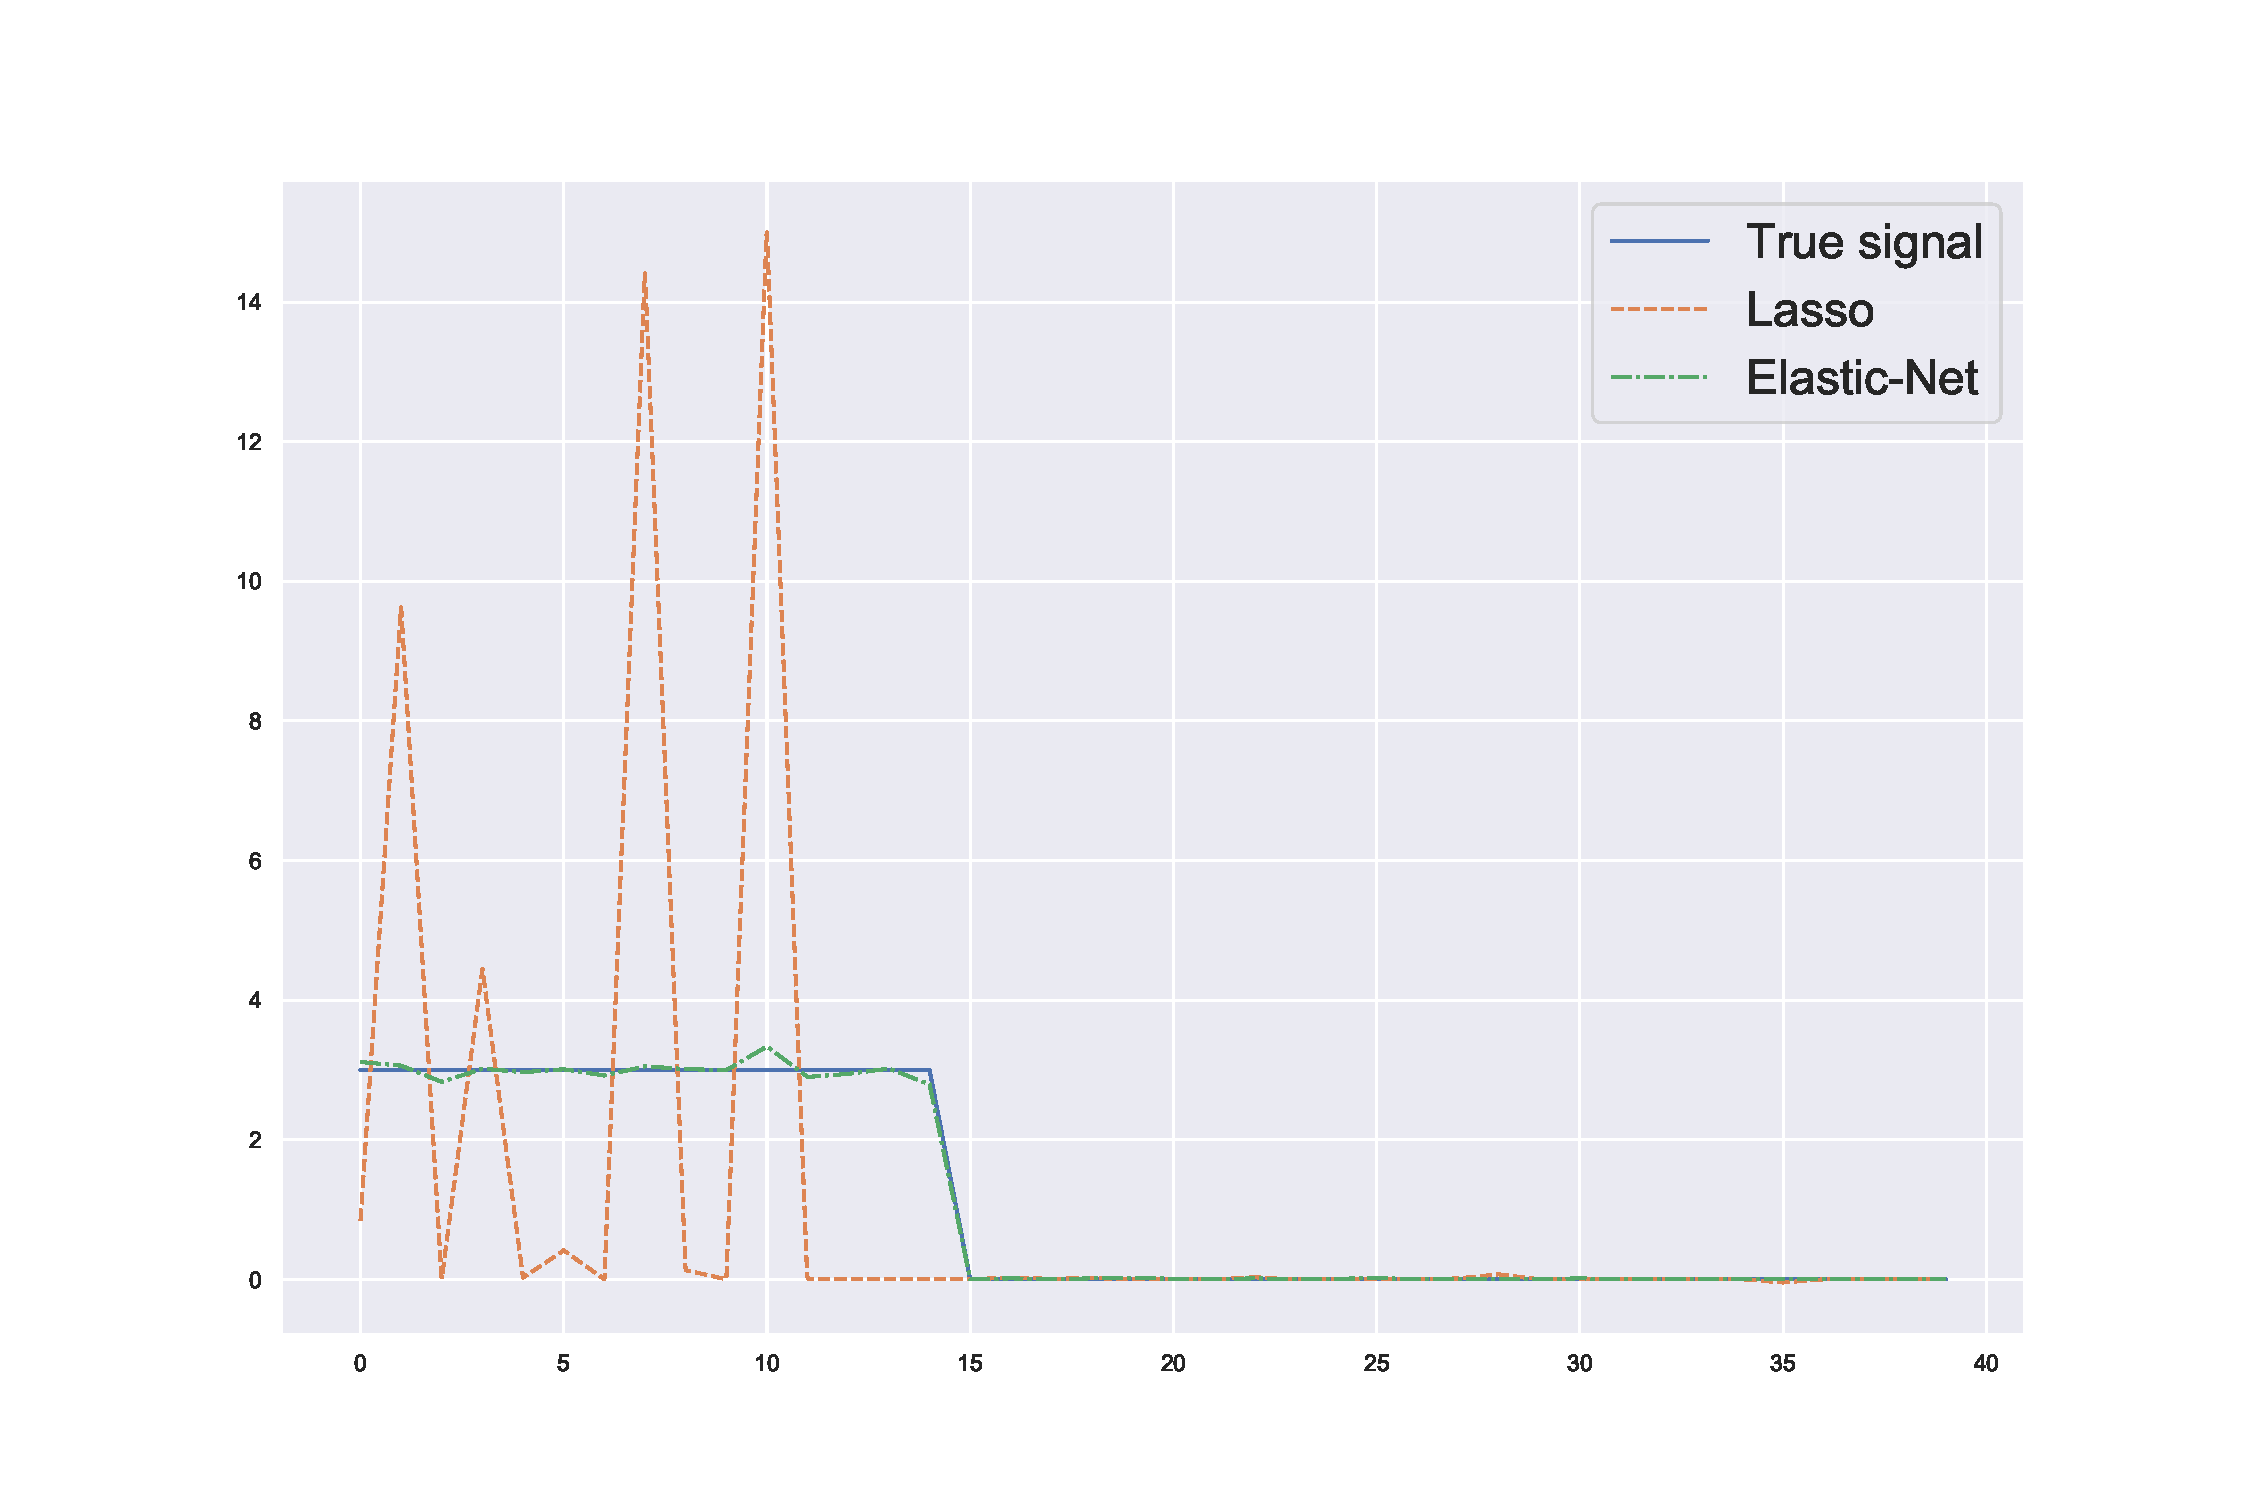
\includegraphics[scale=.23, clip, trim={0cm 0cm 0cm 3.2cm}]{Lasso_enet.pdf} };
    \zoombox[size=2cm]{0.33,0.34}
    \zoombox[width=2cm, height=1cm]{0.65, 0.17}
\end{tikzpicture}


\end{figure}
        \end{onlyenv}
\end{frame}

%%%%%%%%%%%%%%%%%%%%%%%%%%%%%%%%%%%%%%%%%
% Section 1: The proposed regularization
%%%%%%%%%%%%%%%%%%%%%%%%%%%%%%%%%%%%%%%%%

\section[Alternative penalty]{Alternative penalty from the Elastic-net}

\begin{frame}{Penalize with the counting norm}{Introduce the sparse-envelope}

\mytheorem{Definition}
{ The $l_0$ pseudo-norm:
\begin{equation*}
\|x\|_0 = \abs{\{i\,|\, x_i\neq 0\}}
\end{equation*}}
\medskip
\begin{block}{Alternative penalty for a sparse signal}
\[s_k(x):=\mathrm{pen}(x)=\begin{cases}
\frac{1}{2}\|x\|^2_2 & \text{ if }\|x\|_0\leq k\enspace, \\ \infty &\text{ else}\enspace.\end{cases}\]
\end{block}
\end{frame}

%%%%%%%%%%%%%%% The convex biconjugate
\subsection{Visualization of the convex biconjugate}

\begin{frame}{Penalize with the counting norm}{Convex biconjugate}
    \begin{itemize}
    \item \color{red} $s_k$ is not continuous, not differentiable, nor convex.\color{black}
    \item Consider the best convex estimator: $\mathcal{S}_k=s^{**}_k$ where
    \[s_k^*(y)=\max_{x\in\RR^n}\{x'y - s_k(x)\}\enspace.\]
\end{itemize}

\begin{figure}
    \centering
    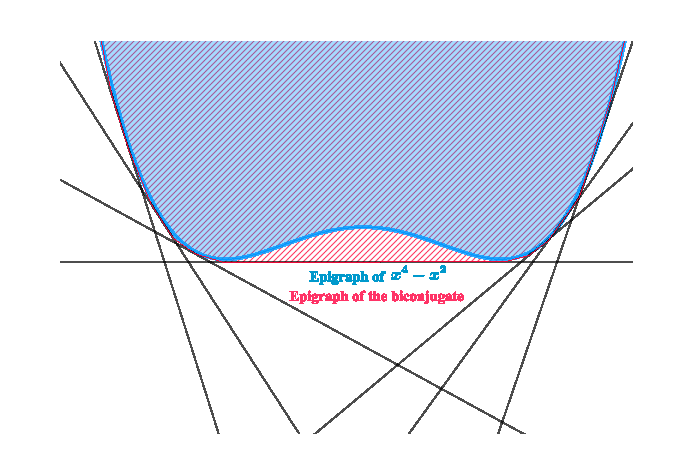
\includegraphics[clip, trim={0cm 2cm 0cm 2cm}]{biconj.pdf}
    \caption{Visualization of the epigraph of the non-convex function $f(x)=x^4-x^2$ and its convex biconjugate $f^{**}(x)$.}
    \label{fig:biconjugate_epigraph}
\end{figure}
\end{frame}

%%%%%%%%%%%%%%%%%%%%%%%%%%%%%%%%%%%%%%%%%%%
%%%%%%%%%%% proximal operator %%%%%%%%%%%%%
%%%%%%%%%%%%%%%%%%%%%%%%%%%%%%%%%%%%%%%%%%%
\section{Compute the proximal operator}
\subsection{Definition}
\begin{frame}{Proximal operator}{}
\begin{itemize}
    \item We now need to solve: $\arg\min_{x\in\RR^n}\|Ax-b\|^2_2 + \lambda \mathcal{S}_k(x)$ \color{red}efficiently\color{black}.
\end{itemize}
\medskip
\mytheorem{Definition}{
    \[\forall x\in\EE,\ \prox_f(x) =\arg\min_{u\in \EE}\left\{ \frac{1}{2}\|u-x\|^2_2 + f(u)\right\}\enspace.\] }
;\medskip
\begin{itemize}
    \item Fast iterative algorithms exist (\emph{eg} FISTA),
    \item Find $\mathcal{S}_k(x)$ is a $n-$dimensional problem.
    \item[\color{red}$\blacktriangleright$\color{black}]<2-> Can we reduce the dimension \textbf{and} use the sparsity?
\end{itemize}
\end{frame}

%%%%%%%%%%%%%%%%%%%%%%%%%%%%%%%%%%%
%%%%%% Reduce dimension %%%%%%%%%%%
%%%%%%%%%%%%%%%%%%%%%%%%%%%%%%%%%%%
\subsection{Reduction of dimension}
\begin{frame}{Proximal operator}{From dimension $n$ to $1$}
    \mytheorem{Theorem}{
\begin{itemize}
    \item If $\|x\|_0\leq k$ then $w=\prox_{\lambda\mathcal{S}_k}(x)=\frac{1}{\lambda + 1}x$,
    \item if $\|x\|_0> k$ then $w_i=(\prox_{\lambda\mathcal{S}_k}(x))_i=\frac{x_iu_i}{\lambda + u_i}$.
\end{itemize}
To find the value of $u_i$, we define $h(\eta)=\sum_{i=1}^n \mathbf{u_i}(\eta) - k$, where the function $\mathbf{u_i}:\eta\mapsto\mathbf{u_i}(\eta)$ is:
\[\mathbf{u_i}(\eta)=\begin{cases}
0 & \text{ if }\eta \leq \frac{\lambda}{\abs{x_i}}\enspace,\\
\abs{x_i}\eta & \text{ if }\frac{\lambda}{\abs{x_i}}< \eta < \frac{\lambda  + 1}{\abs{x_i}}\enspace,\\
1 & \text{ if } \eta\geq \frac{\lambda+1}{\abs{x_i}}\enspace,
\end{cases} i=1,\dots,n\enspace.
\]
Then $u_i=\mathbf{u_i}(\tilde\eta)$, with $\tilde\eta$ defined such that $h(\tilde\eta)=0$.
}
\begin{itemize}
    \item<2-> \color{red} Find the root of the sum of $n$ piecewise linear functions with two breakpoints $\Longrightarrow$ \textit{Random Search} algorithm or bisector method.
\end{itemize}
\end{frame}

%%%%%%%%%%%%%%%%%%%%%%%%%%%%%%%%%%%
%%%%%%%%% Compare paths and signals
%%%%%%%%%%%%%%%%%%%%%%%%%%%%%%%%%%%

\subsection{Comparisons of our methods}

% Compare the signals obtained
\begin{frame}{Elastic-net and sparse-envelope}{Obtained signals}
\begin{figure}
\captionsetup[subfigure]{labelformat=empty}
\begin{tikzpicture}[
    zoomboxarray,
    zoomboxarray columns=1,
    zoomboxarray rows=2,
    connect zoomboxes,
    zoombox paths/.append style={line width=1pt}
]
    \node [image node] { 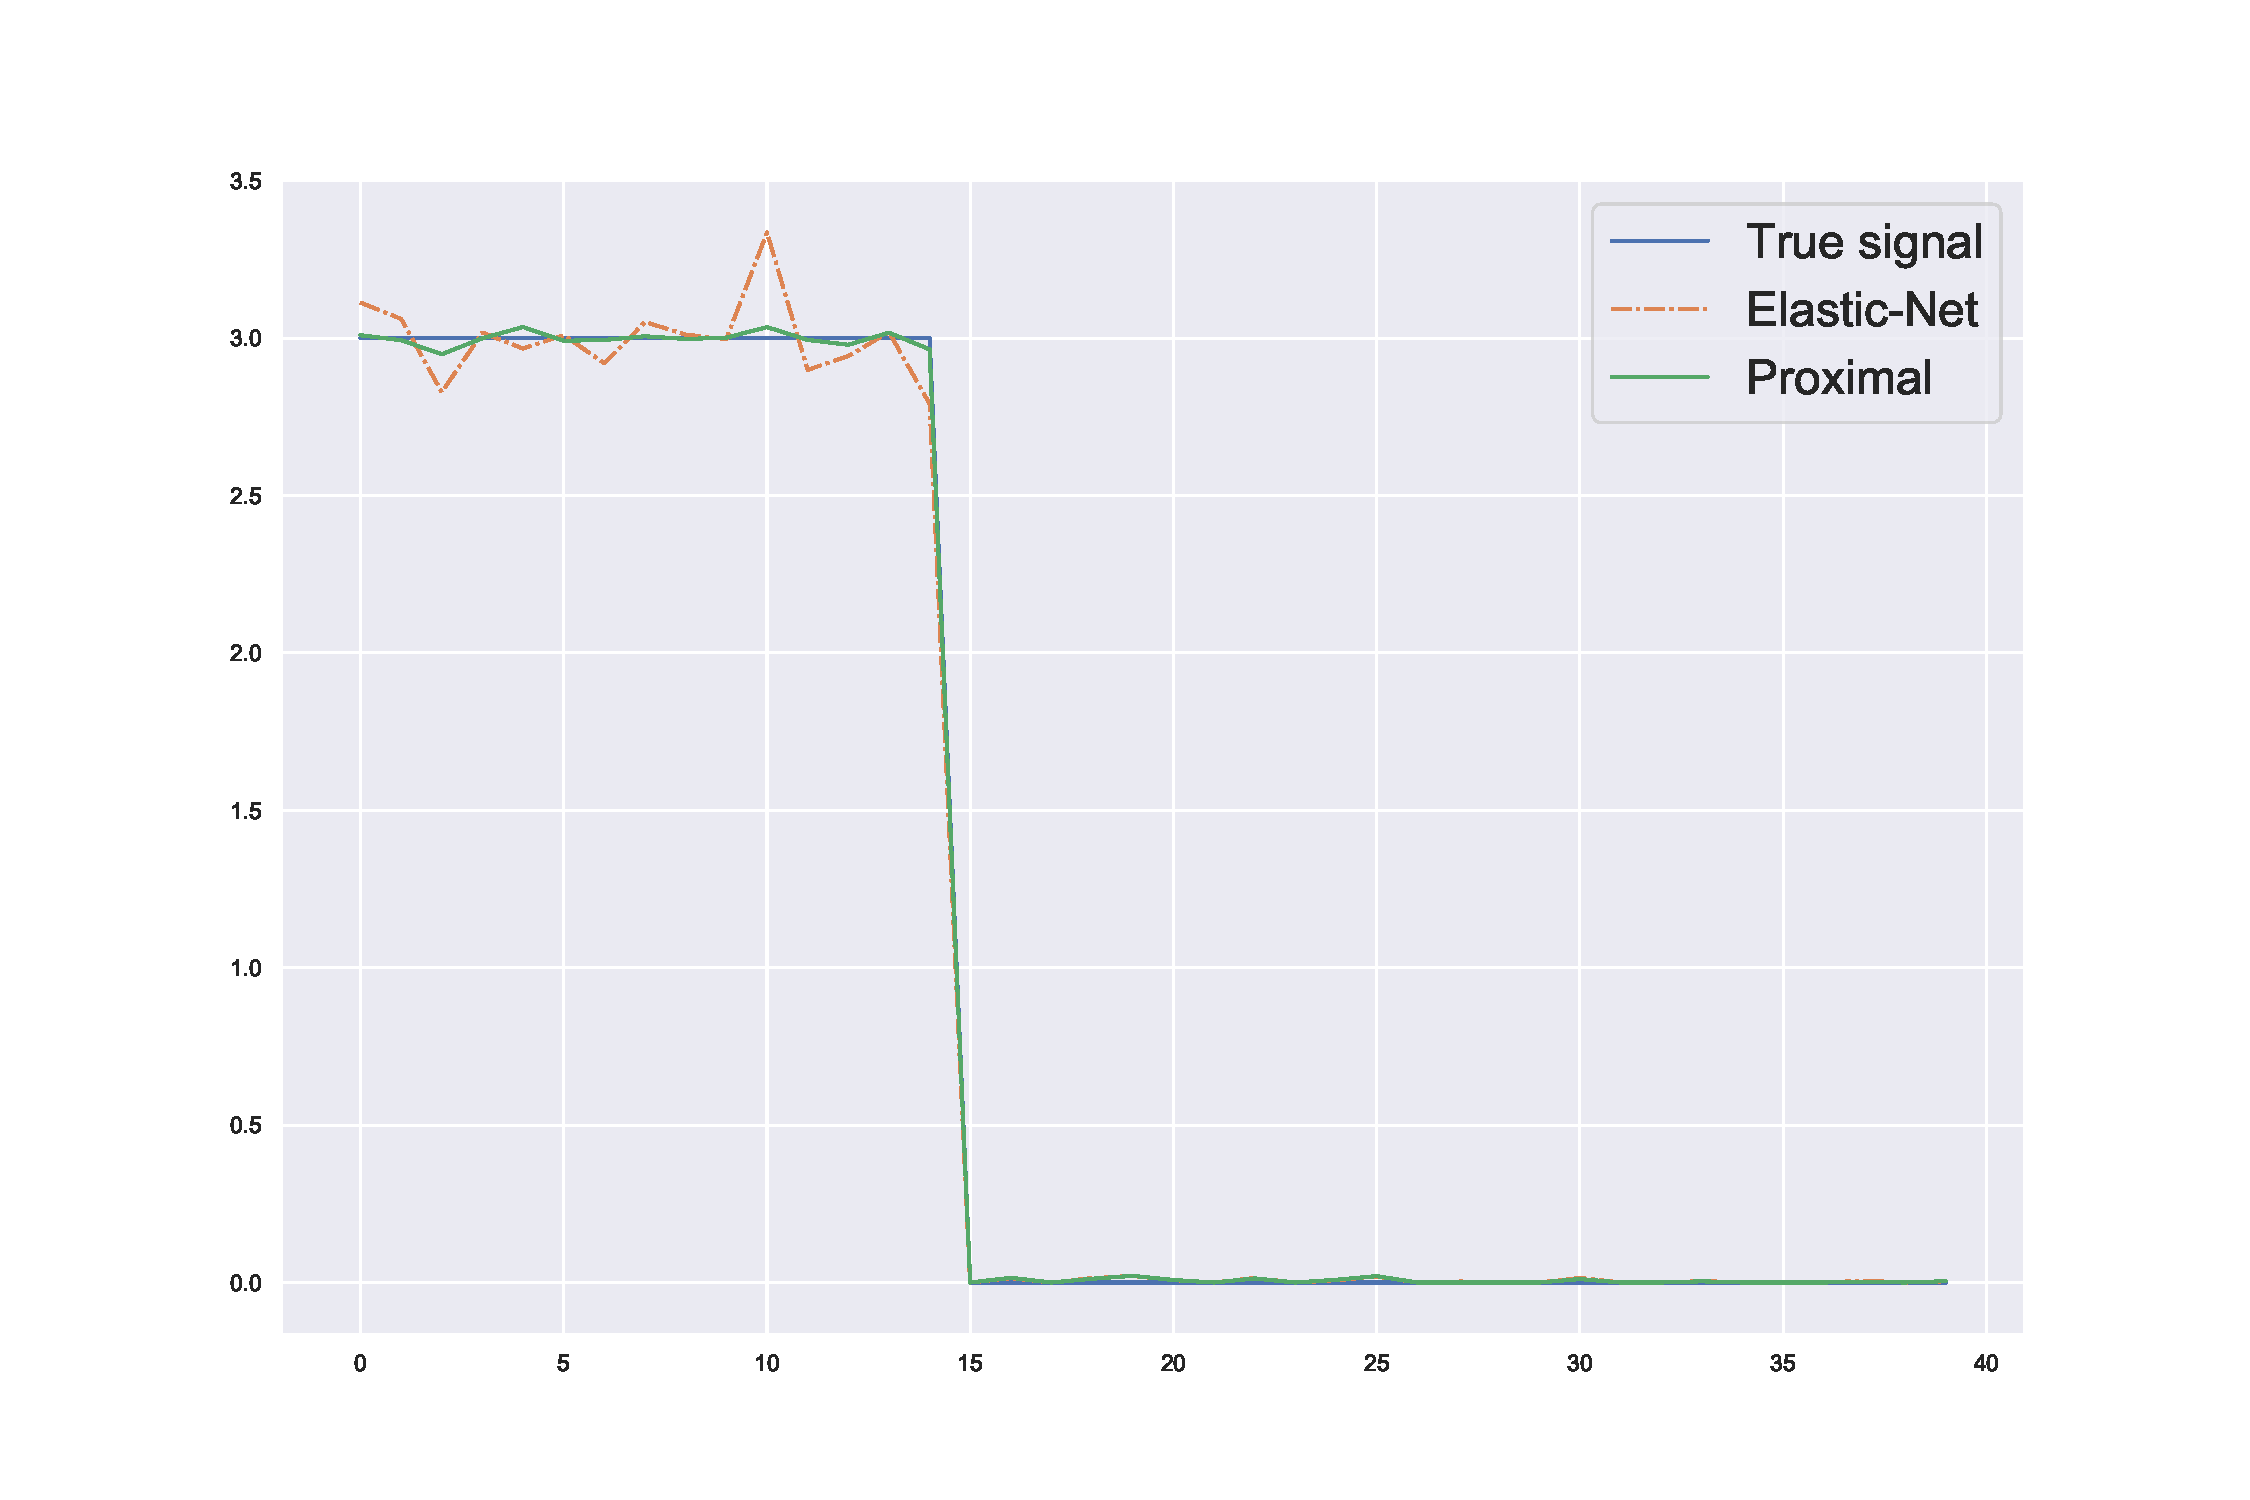
\includegraphics[scale=.23, clip, trim={0cm 2cm 0cm 3.2cm}]{enet_proxi.pdf} };
    \zoombox[size=2cm]{0.33,0.9}
    \zoombox[width=2cm, height=1cm]{0.7, 0.1}
\end{tikzpicture}

\caption{\enet and \textbf{sparse envelope} with highly correlated groups of variables.}
\end{figure}
\end{frame}

% Compare the coeficients

\begin{frame}{Elastic-net and sparse-envelope}{Coefficients paths}
\begin{center}
\begin{figure}
  \begin{minipage}[c]{0.67\textwidth}
   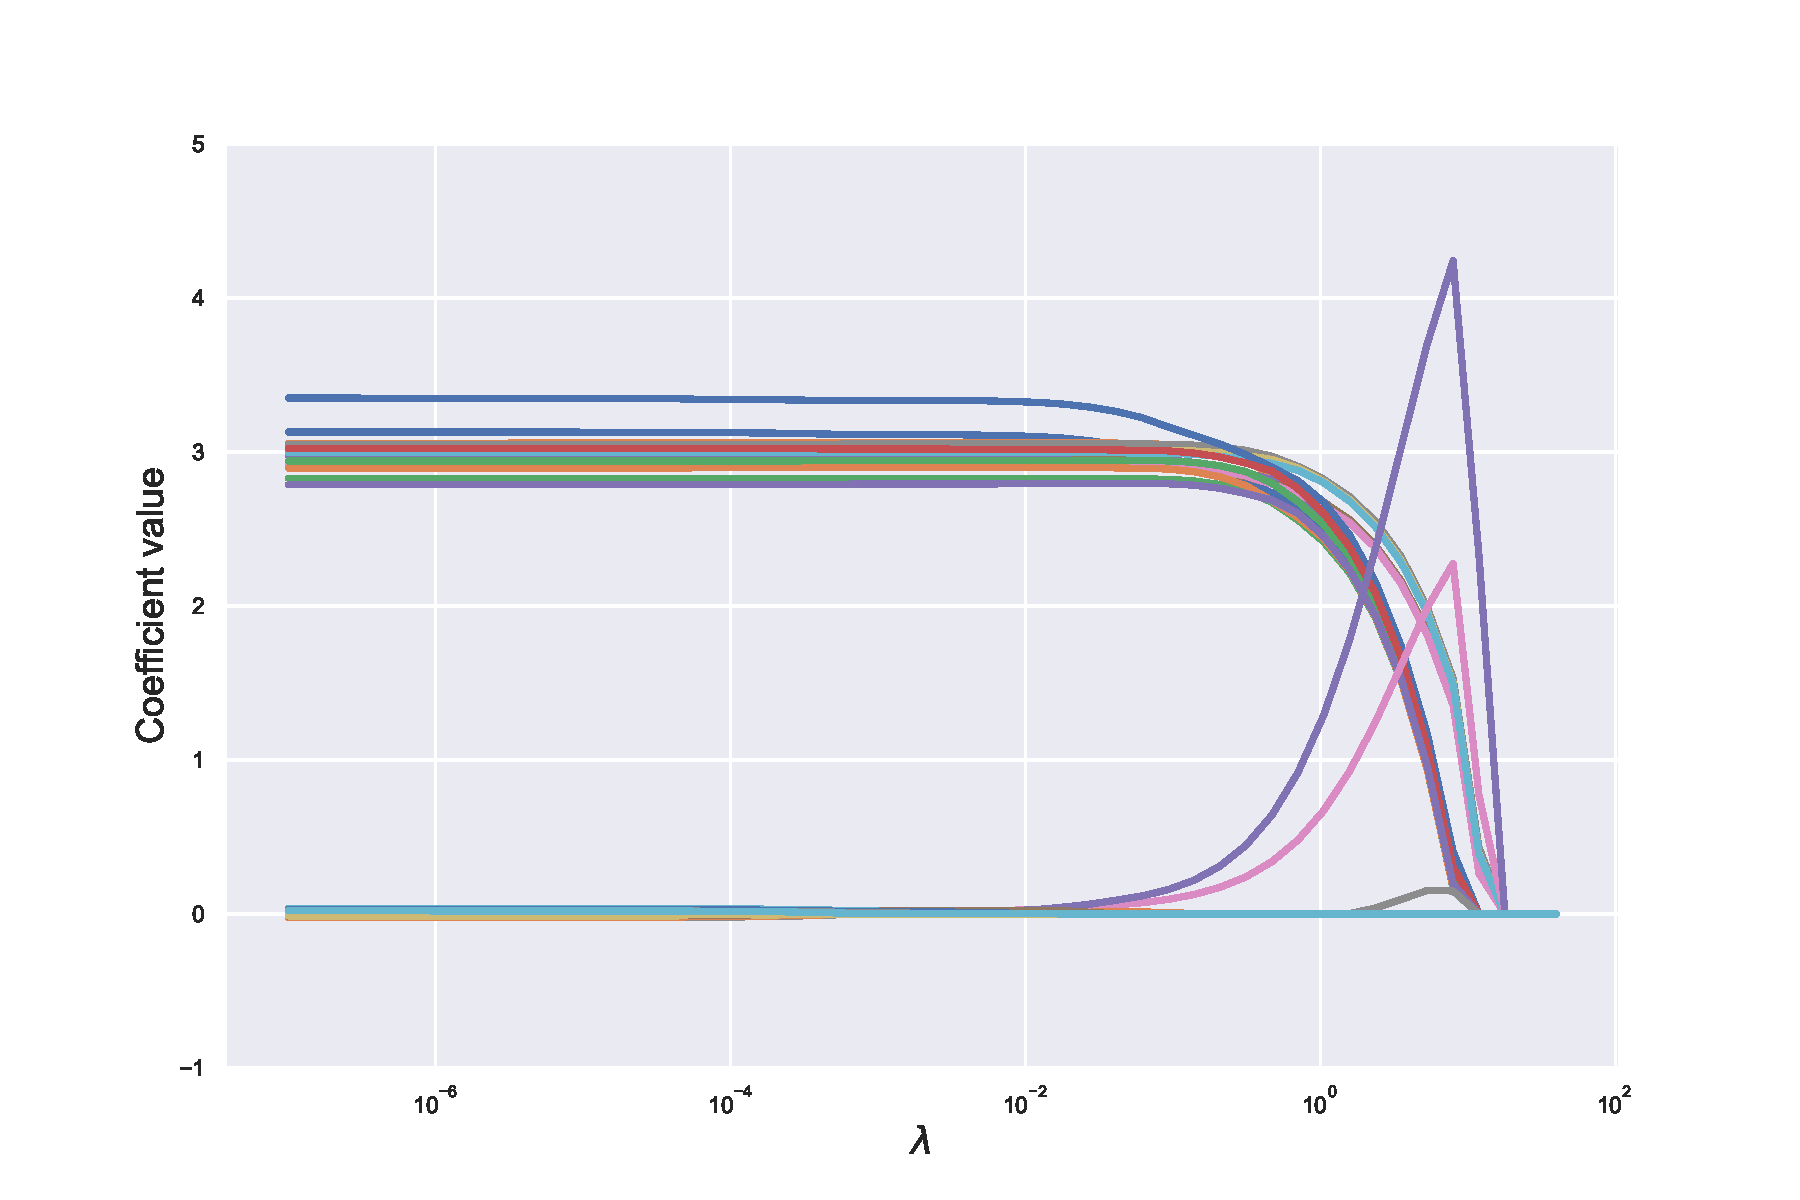
\includegraphics[height=3cm, width=8cm, clip, trim={0cm .5cm 0cm 2.2cm}]{enet_coeffs.pdf}
   \end{minipage}\hfill
  \begin{minipage}[c]{0.3\textwidth}
    \caption{
   Path of the coefficients for each $\lambda$ for the \enet with a $l_1$ ratio determined by K-fold validation.
    }
  \end{minipage}
\end{figure}

\begin{figure}
  \begin{minipage}[c]{0.67\textwidth}
   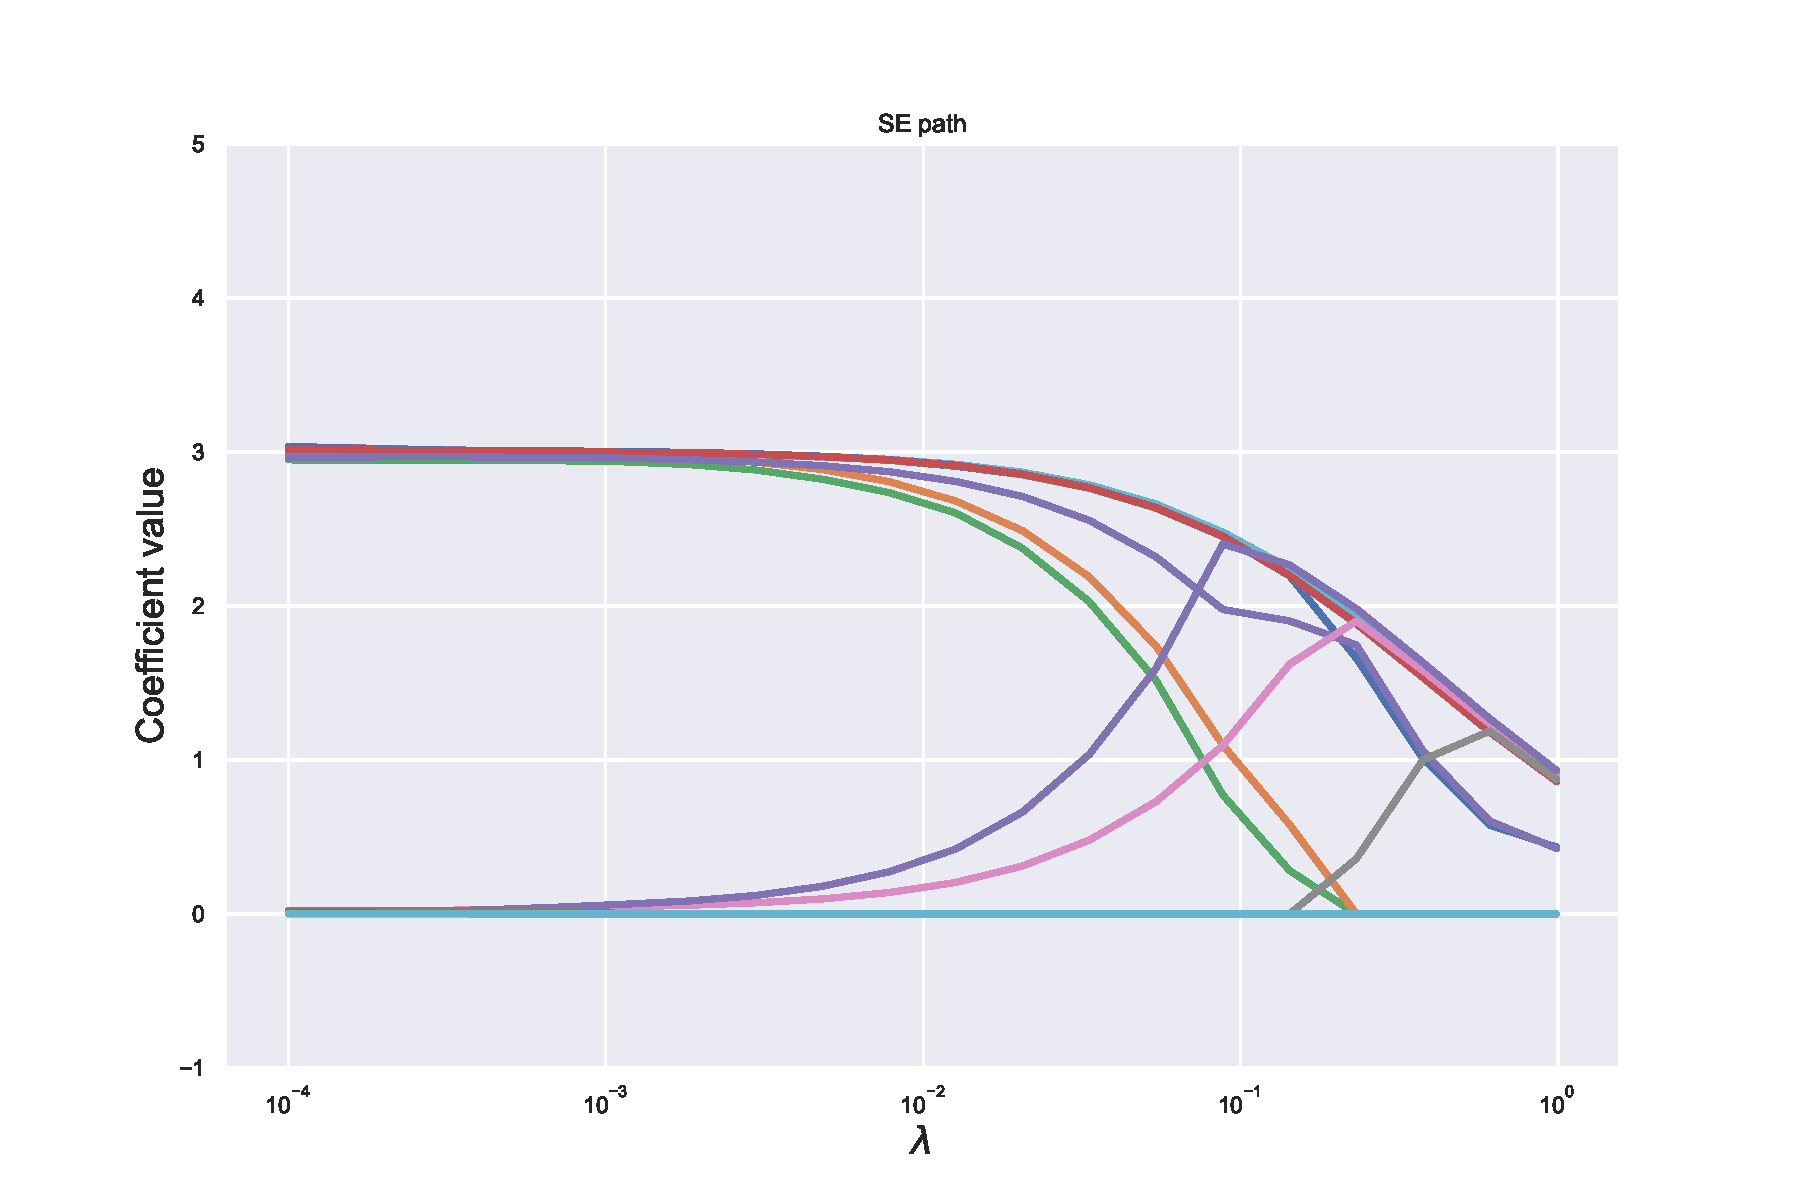
\includegraphics[height=3cm, width=8cm, clip, trim={0cm .5cm 0cm 2.2cm}]{se_coeffs.pdf}
   \end{minipage}\hfill
  \begin{minipage}[c]{0.3\textwidth}
    \caption{
      Path of the coefficients for each $\lambda$ for the \textbf{sparse envelope} with $k=15$ predetermined.
    }
  \end{minipage}
\end{figure}
\end{center}
\end{frame}

% What if k is not known?
\begin{frame}{Elastic-net and sparse-envelope}{For k sub or over optimal}
\begin{figure}
    \captionsetup[subfigure]{labelformat=empty}
\begin{tikzpicture}[
    zoomboxarray,
    zoomboxarray columns=1,
    zoomboxarray rows=2,
    connect zoomboxes,
    zoombox paths/.append style={line width=1pt}
]
    \node [image node] { 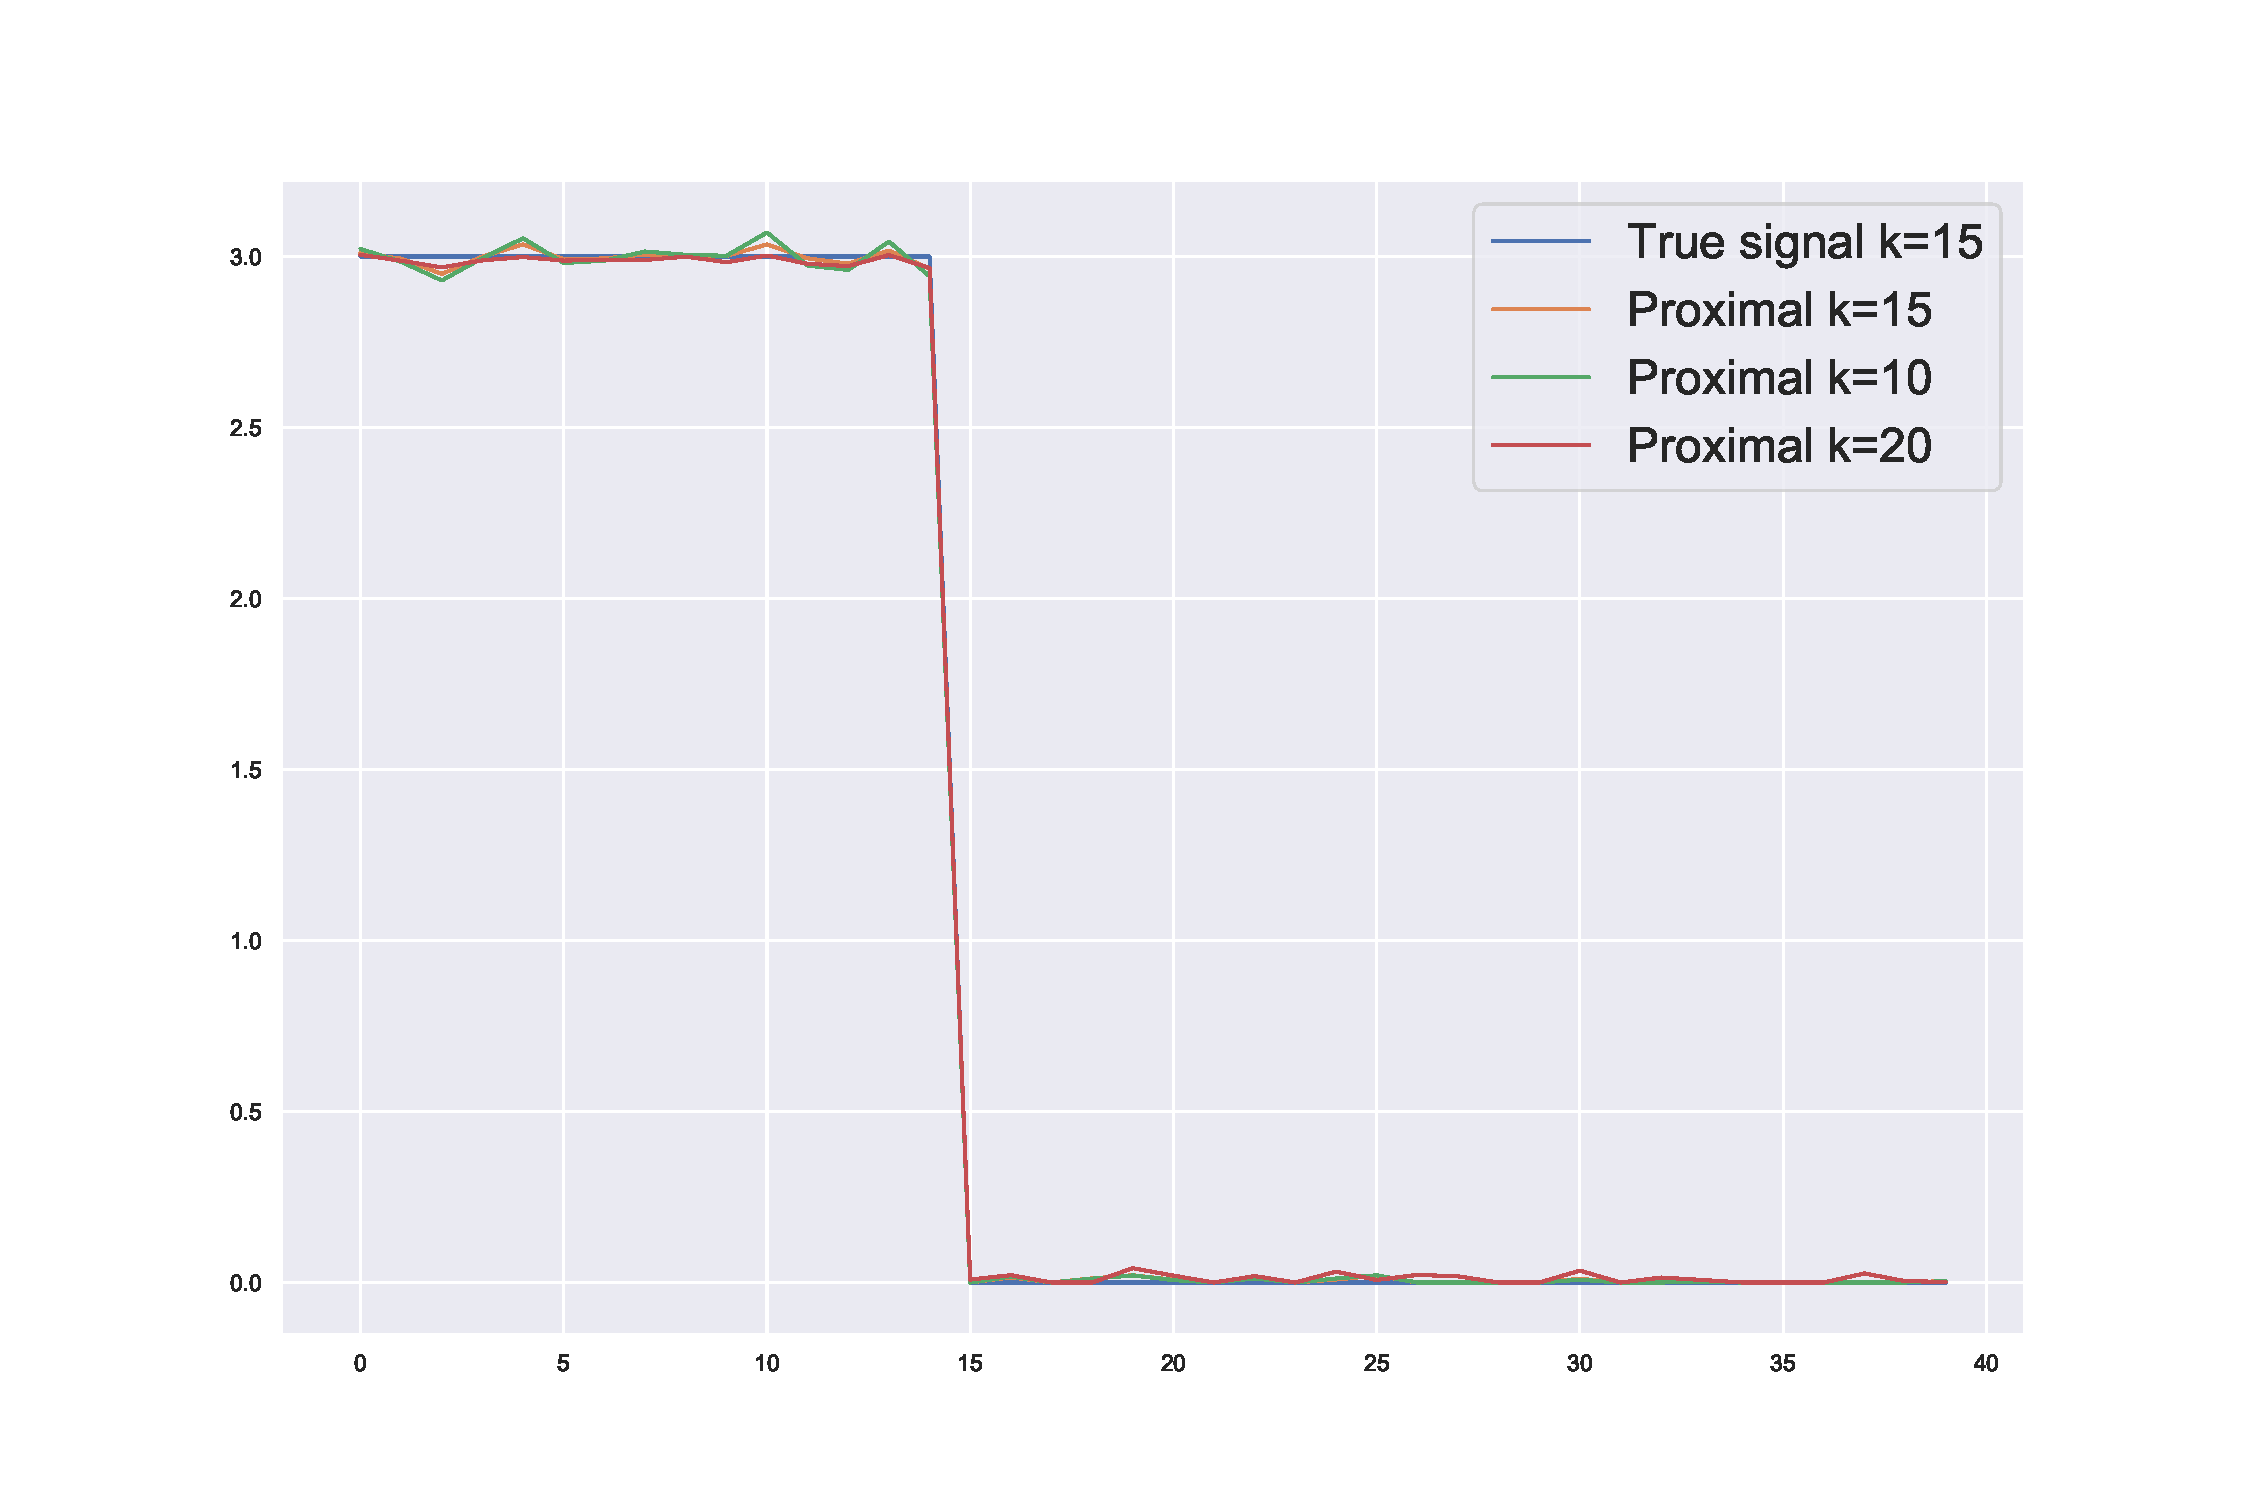
\includegraphics[scale=.23, clip, trim={0cm 2cm 0cm 3.2cm}]{proxi_diff_k.pdf} };
    \zoombox[width=2.5cm, height=1cm]{0.33,0.95}
    \zoombox[width=2cm, height=1cm]{0.7, 0.1}
\end{tikzpicture}

\caption{Comparison of the signal obtained from the sparse envelope when the level of sparsity is not known in advance.}
\end{figure}
\end{frame}

%%%%%%%%%%%%%%%%%%%%%%%%%%%%
% Conclusion and biblio
%%%%%%%%%%%%%%%%%%%%%%%%%%%%
\section{Conclusion}
\begin{frame}{Conclusion}
    \begin{itemize}
      \setlength\itemsep{1em}
        \item<1-> Visible improvements for the signal in output,
        \item<1-> fast methods that take into account the sparsity in the computation,
        \item<2-> \color{red} penalty that is natural and easy to interpret,
        \item<2-> \color{red}so is the obtained signal if there is not a lot of coefficients.\color{black}
    \end{itemize}
\end{frame}

%%%%%% bibliography
\begin{frame}{Bibliography}
\setbeamertemplate{bibliography item}{\insertbiblabel}
\nocite{*}
\printbibliography[heading=none]
\end{frame}

\begin{frame}[plain,noframenumbering]
	\standoutpage{\bfseries\huge Thank you!}
\end{frame}

\end{document}
